% =========================================================================
\FloatBarrier
\section{Case Study: The London Ambulance Service}
\label{sec:exp-emergency}
% =========================================================================

The London Ambulance Service (LAS) is the busiest urban ambulance service in the United Kingdom. It serves about $9$ million residents through $66$ ambulance stations organized into $21$ operational Groups within $5$ sectors. Optimization studies of LAS produce a single recommended plan~\citep{mccormack2015simulation}. We instead run FalCom on the real stations, with no artificial candidates, to obtain a reference distribution over hierarchical layouts, and we use it in three ways.
\begin{itemize}[leftmargin=1.5em,itemsep=1pt,topsep=3pt]
\item \emph{Structure} (Section~\ref{sec:las-structure}). The ensemble separates settled from contested geography: $12\%$ of adjacencies are almost never cut by a station boundary, and $59\%$ of small areas have no station that serves them in even half of the plans.
\item \emph{Stations and Groups} (Section~\ref{sec:las-structure}). A sampled plan opens $52.5$ of the $66$ stations on average; $17$ stations are open in more than $90\%$ of plans and none in fewer than $40\%$. The real Groups are a typical member of the sampled groupings, not their mode.
\item \emph{The operational layout} (Section~\ref{sec:las-price}). The operational layout has a lower access cost than every sampled plan, because $20$ of its $66$ stations carry loads that no balanced plan allows. The best balanced plan we found is $0.5$ minutes of mean drive time away from it, which bounds from above what workload balance would cost in access at this calibration.
\end{itemize}
The convergence diagnostics of the London chains are in Table~\ref{tab:multistart} and their rejections in Table~\ref{tab:rejections}; Section~\ref{sec:las-sensitivity} repeats the study under a second demand proxy and a wider tolerance.

% -------------------------------------------------------------------------
\subsection{Instance, Calibration and Benchmark}\label{sec:las-data}
% -------------------------------------------------------------------------

\paragraph{Data.}
The base graph $G^1$ has $|V^1| = 4{,}994$ nodes, the Lower layer Super Output Areas (LSOAs) of Greater London on 2021 boundaries, joined by $|E^1| = 14{,}550$ rook-adjacency edges (Figure~\ref{fig:las-instance}). LSOAs are the small-area unit of NHS planning and of recent spatial work on LAS~\citep{murphy2024socio}. The candidate set $F^1$ is the set of $66$ LSOAs that contain an active station, and any open station can serve as the level-2 facility of its superdistrict. Demand $d_v$ is the annual number of attended incidents: the 2010 to 2015 mean of the borough totals that LAS publishes~\citep{las_incidents}, about $1.056$ million incidents a year, apportioned to the LSOAs of each borough in proportion to population~\citep{ons_sape2024}. Travel times are shortest-path driving times on the OpenStreetMap road network from every station to every LSOA centroid, with free-flow speeds scaled by $1.6$ for driving under lights and sirens. Variation within a borough is thus a proxy, and the speed factor is an assumption; Section~\ref{sec:las-sensitivity} tests the proxy and Appendix~\ref{app:slas} documents the assembly.

\begin{figure}[!htbp]
\centering
\begin{subfigure}[t]{0.495\linewidth}
  \centering
  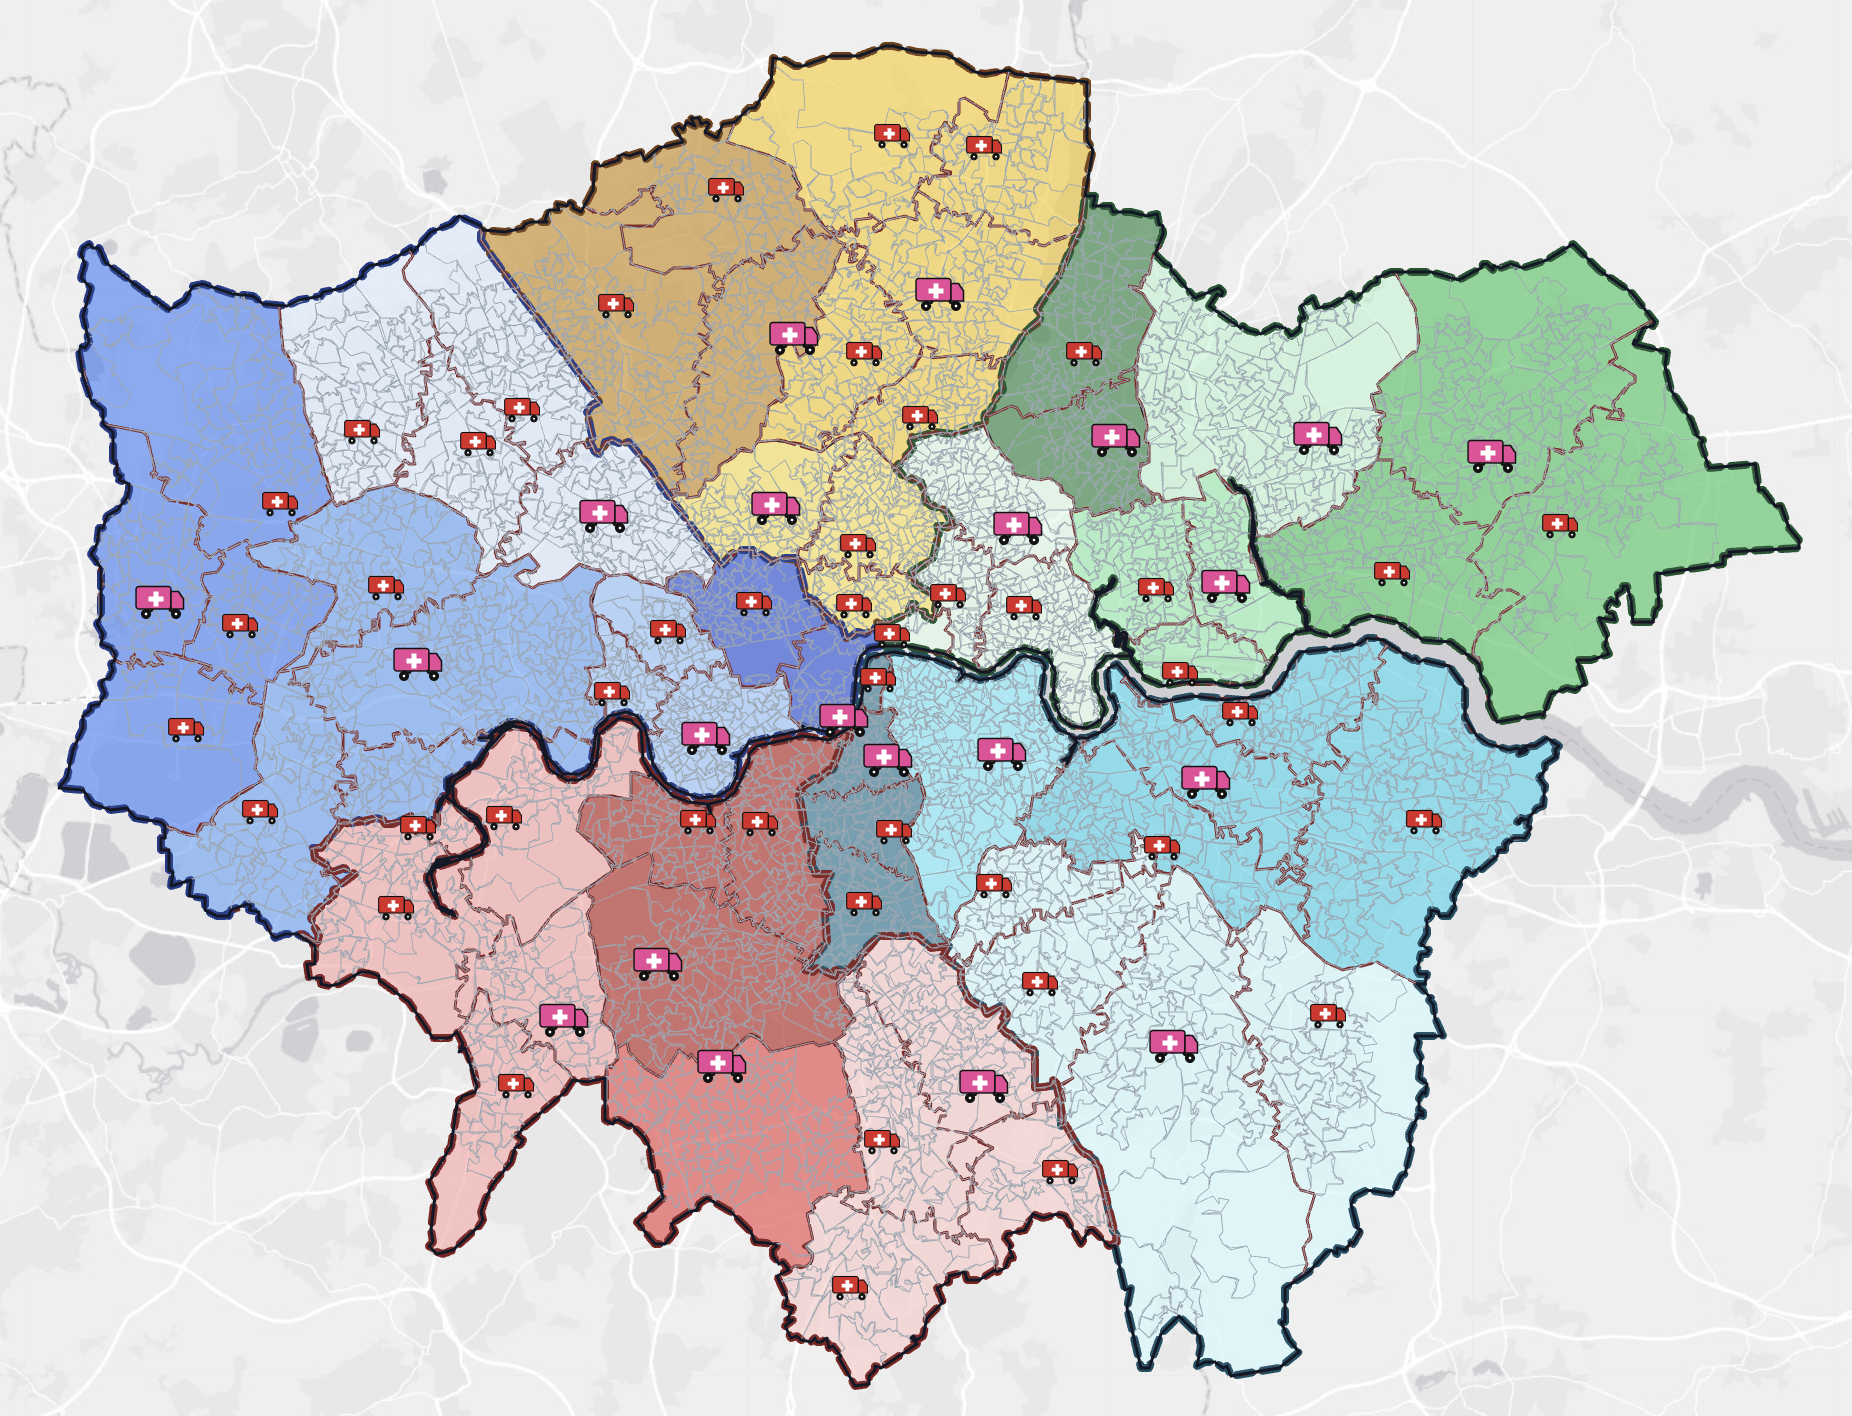
\includegraphics[width=\linewidth]{figures/las_map.png}
  \caption{LSOA polygons of the LAS catchment with the stations.}
  \label{fig:las-lsoas}
\end{subfigure}
\hfill
\begin{subfigure}[t]{0.495\linewidth}
  \centering
  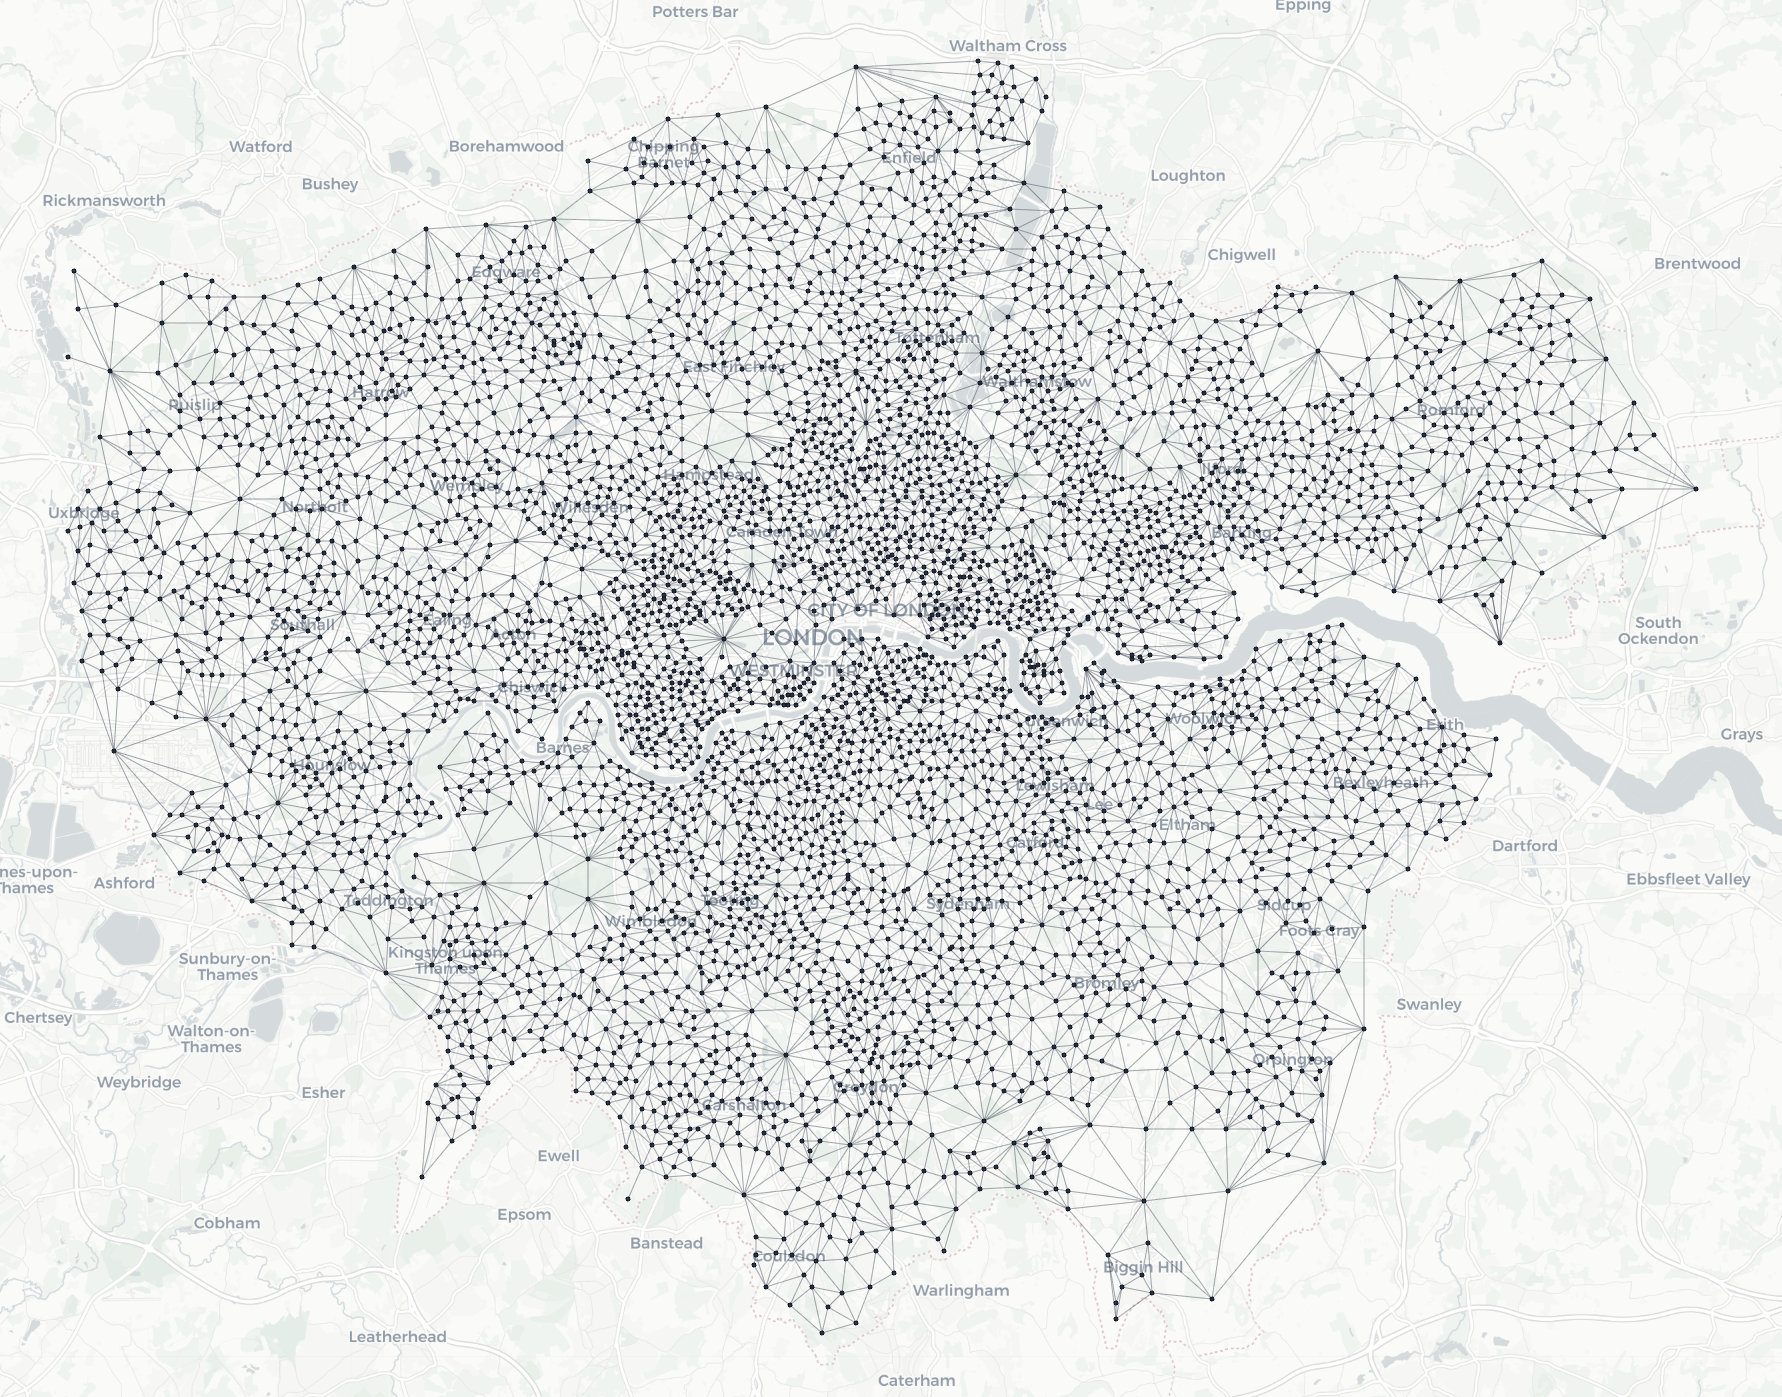
\includegraphics[width=\linewidth]{figures/las_dual_graph.png}
  \caption{Rook-adjacency dual graph $G^1$, $14{,}550$ edges.}
  \label{fig:las-dual}
\end{subfigure}
\caption{The LAS instance. The $48$ Brentwood LSOAs, served by another ambulance service, are excluded. Each node of the dual graph carries its integer annual demand.}
\label{fig:las-instance}
\end{figure}

\paragraph{Calibration.}\label{sec:las-calibration}
The capacity unit is a block of ambulances. The 2024/25 Annual Report~\citep{las_ar_2024_25} states a target of $5.2$ patients per crew per twelve-hour shift; five patients per shift, two shifts a day and $365$ days give $3{,}650$ calls per ambulance per year. The granularity floor requires the per-unit tolerance $\varepsilon^1 w$ to exceed the heaviest LSOA demand, $1{,}526$, so a unit must hold at least three ambulances. We take blocks of three, $w = 10{,}887$ calls per year, and the catchment's demand is $k = 97$ units, which every sampled state carries exactly. Stations carry one to three units, the safe range of Corollary~\ref{cor:app-invariant}, and Groups carry two to six units in at least two stations. By Proposition~\ref{prop:effective} a sampled one-unit station then serves between $0.72$ and $1.32$ units, a two-unit station between $1.51$ and $2.56$ and a three-unit station between $2.29$ and $3.79$. The number of open stations is not an input: the calibration admits between $33$ and $66$, and the chain decides. The unit is a demand quantum and not a vehicle count, since the fleet of April 2025 is about twice the $291$ vehicles that $97$ blocks at the published target would be; a calibration that bounds each station by the fleet based there is left to future work.

\paragraph{Readouts.}
Energy plays no part in the sampling. On the samples we evaluate the station leg of the median energy,
\[
  E_1(s) \;=\; \sum_{D \in \Pc^1} \sum_{v \in D} d_v \, t\bigl(v, f^1(D)\bigr),
\]
in demand-weighted minutes, the drive-time form of the level-1 term of objective~\eqref{eq:milp-median}, and three metrics of the same static assignment of every LSOA to its catchment station: the demand-weighted mean drive time, its $90$th percentile, and the share of demand within eight minutes' drive. The Group leg $E_2$, the corresponding sum to the level-2 facility, is a measure of how compactly the stations of a superdistrict sit around their most central member. It is not a dispatch distance, since LAS dispatches from two Emergency Operations Centres, and we do not use it in the comparison with the operational layout, whose Groups have fixed headquarters.

\paragraph{The operational layout.}
We reconstruct the current operational layout as a state $s_{\mathrm{LAS}}$ in the same space (Figure~\ref{fig:las-plan}a). Sectors are unions of boroughs; the list of departments~\citep{las_departments2025} and the 2023 operational estate map~\citep{las_estate2023} assign each LSOA to a Group; and within a Group every LSOA is served by its nearest station. All $66$ catchments and all $21$ Groups are connected on $G^1$ (Appendix~\ref{app:slas}). The layout is not a member of the sampled space, for two reasons that are themselves findings. Three Groups (Deptford, Ilford and St Helier) contain a single station, which $\kappa^2_{\min} = 2$ forbids, and the station loads range from $0.19$ to $4.68$ units, far outside the balance windows. The Group loads, $2.0$ to $6.7$ units, lie inside the level-2 windows.

\paragraph{Runs.}\label{sec:las-protocol}
Four chains run for $80{,}000$ steps each from sector-wise initial plans, and a fifth from a Group-based plan (Section~\ref{sec:exp-multistart}). A chain takes $61$ to $62$ minutes on one core. The full plan is stored every $40$ steps and the first $16{,}000$ steps are discarded, so the pooled ensemble of the four chains holds $6{,}400$ plans, worth about $1{,}800$ independent draws for the slowest observables (Table~\ref{tab:multistart}). Readouts computed per chain agree: the open frequency of a station differs between two chains by at most $0.08$, with a Monte Carlo standard error of at most $0.016$ (Appendix~\ref{app:london-extra}).

\begin{figure}[!htbp]
\centering
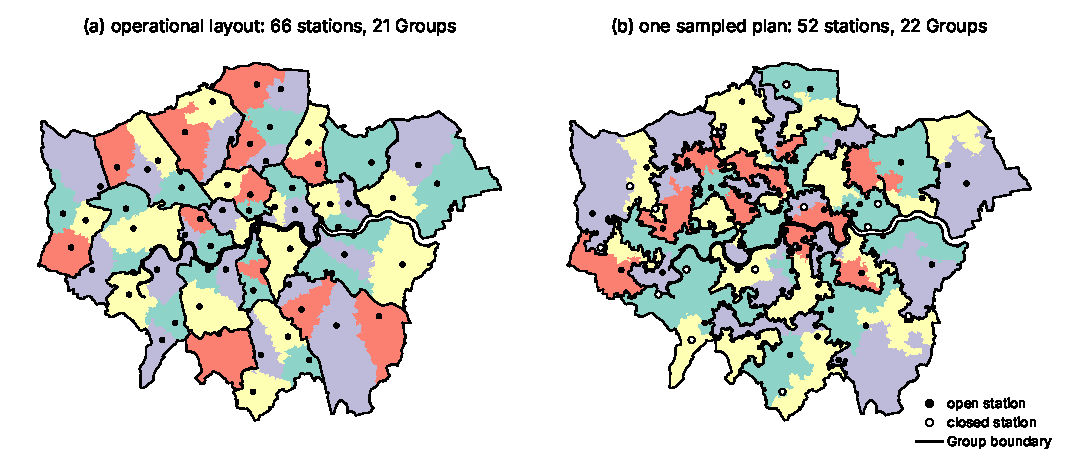
\includegraphics[width=\linewidth]{figures/sec7/fig_plan_vs_layout.pdf}
\caption{(a) The operational layout $s_{\mathrm{LAS}}$: $66$ station catchments in $21$ Groups. (b) One sampled plan, the last stored plan of the first chain. Colours distinguish neighbouring station catchments and carry no other meaning.}
\label{fig:las-plan}
\end{figure}

% -------------------------------------------------------------------------
\FloatBarrier
\subsection{What Most Sampled Plans Have in Common}\label{sec:las-structure}
% -------------------------------------------------------------------------

\paragraph{What a frequency means.}
Every frequency below estimates a probability under the stationary law of the chain as implemented, with its rejection rule and retry budget. That law is characterized only empirically. It is supported on plans that satisfy the windows and it is not uniform over them (Section~\ref{sec:exp-enumeration}). The readouts therefore come in three kinds. Statements about the operational layout, its loads and its position relative to every sampled plan, do not depend on the law. Frequencies, how often an edge is cut, a station open or two stations grouped, do, and Sections~\ref{sec:exp-ablation} and~\ref{sec:las-sensitivity} show how they respond to the retry budget, the tolerance and the demand proxy. Group readouts depend in addition on the greedy supergraph recursion, whose law is validated against enumeration only on small instances.

\paragraph{Boundaries.}
The ensemble separates the geography that most sampled plans reproduce from the choices that remain open (Figure~\ref{fig:las-boundary}). Over the $6{,}400$ plans, no edge of $G^1$ is cut by a station boundary in more than $44\%$ of them. $12.1\%$ of the $14{,}550$ edges are cut in fewer than $10\%$ of plans and lie inside catchments in nearly every plan; the other $87.9\%$ are contested. Group boundaries are more constrained: $30.8\%$ of edges are interior at level $2$, no edge is cut in more than $34\%$ of plans, and the level-2 boundary frequency concentrates on a few corridors in inner north London and along the river. Seen from the units, an LSOA is served by its most frequent station in $48.3\%$ of plans on average, and $58.9\%$ of LSOAs have no station that serves them in even half of the plans. The map of contestedness shows a settled core around each station, contested ground between stations, and settled fringes where stations are scarce (Heathrow, Havering, the southern edge), which are settled by scarcity and not by geography.

\begin{figure}[!htbp]
\centering
\begin{subfigure}[t]{\linewidth}
  \centering
  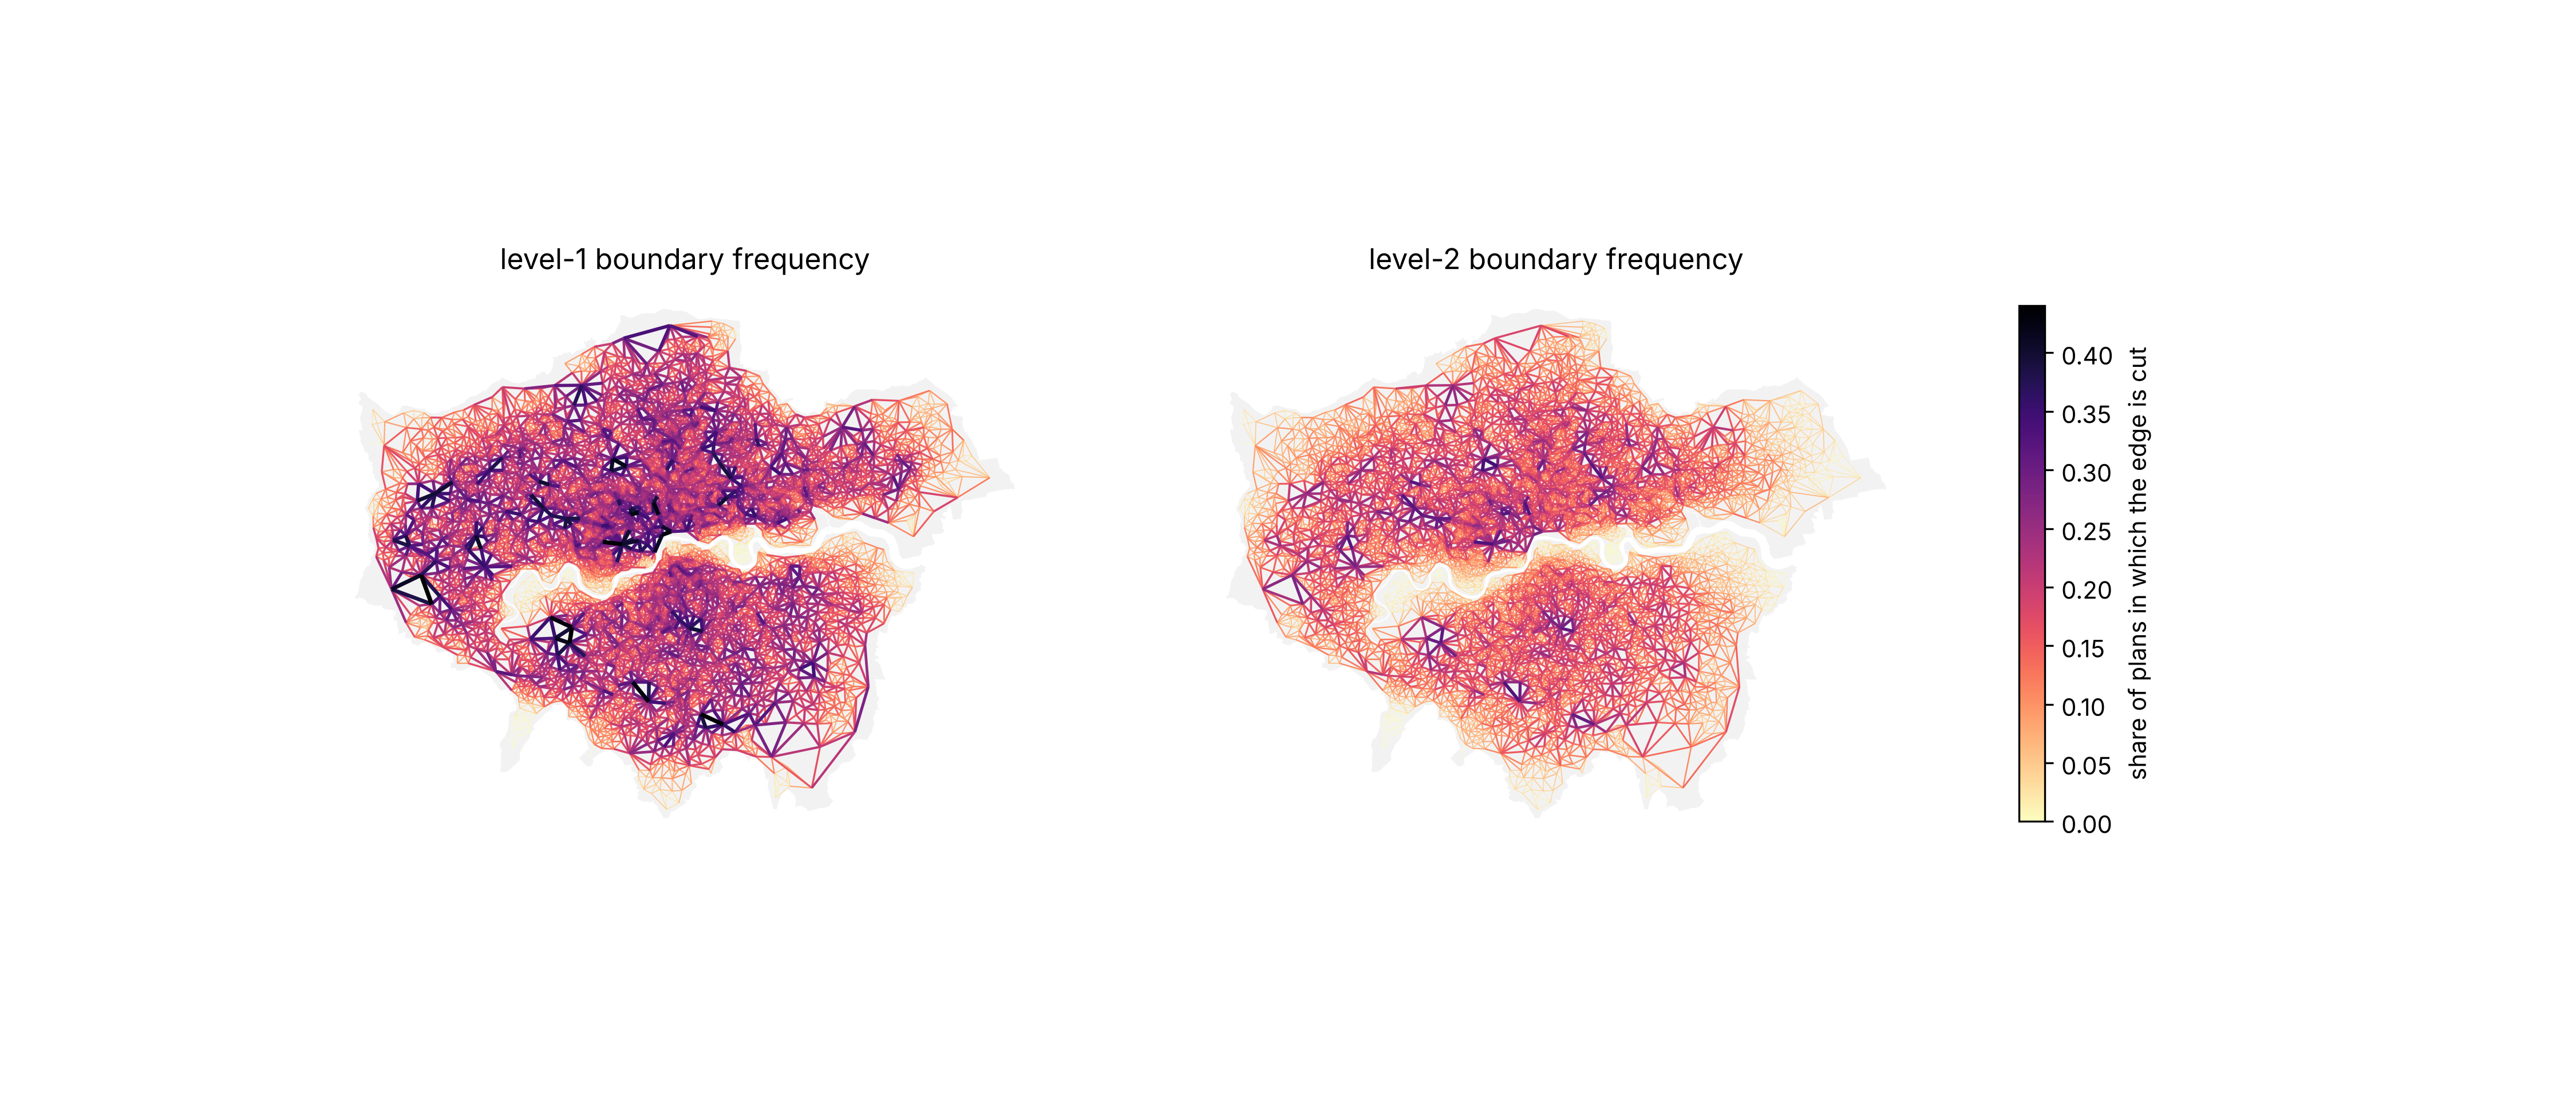
\includegraphics[width=\linewidth,trim=0 80 0 80,clip]{figures/las/fig_boundary_freq.png}
  \caption{Share of plans in which each edge of $G^1$ is cut by a station boundary (left) or a Group boundary (right).}
  \label{fig:las-boundary-panels}
\end{subfigure}

\begin{subfigure}[t]{0.55\linewidth}
  \centering
  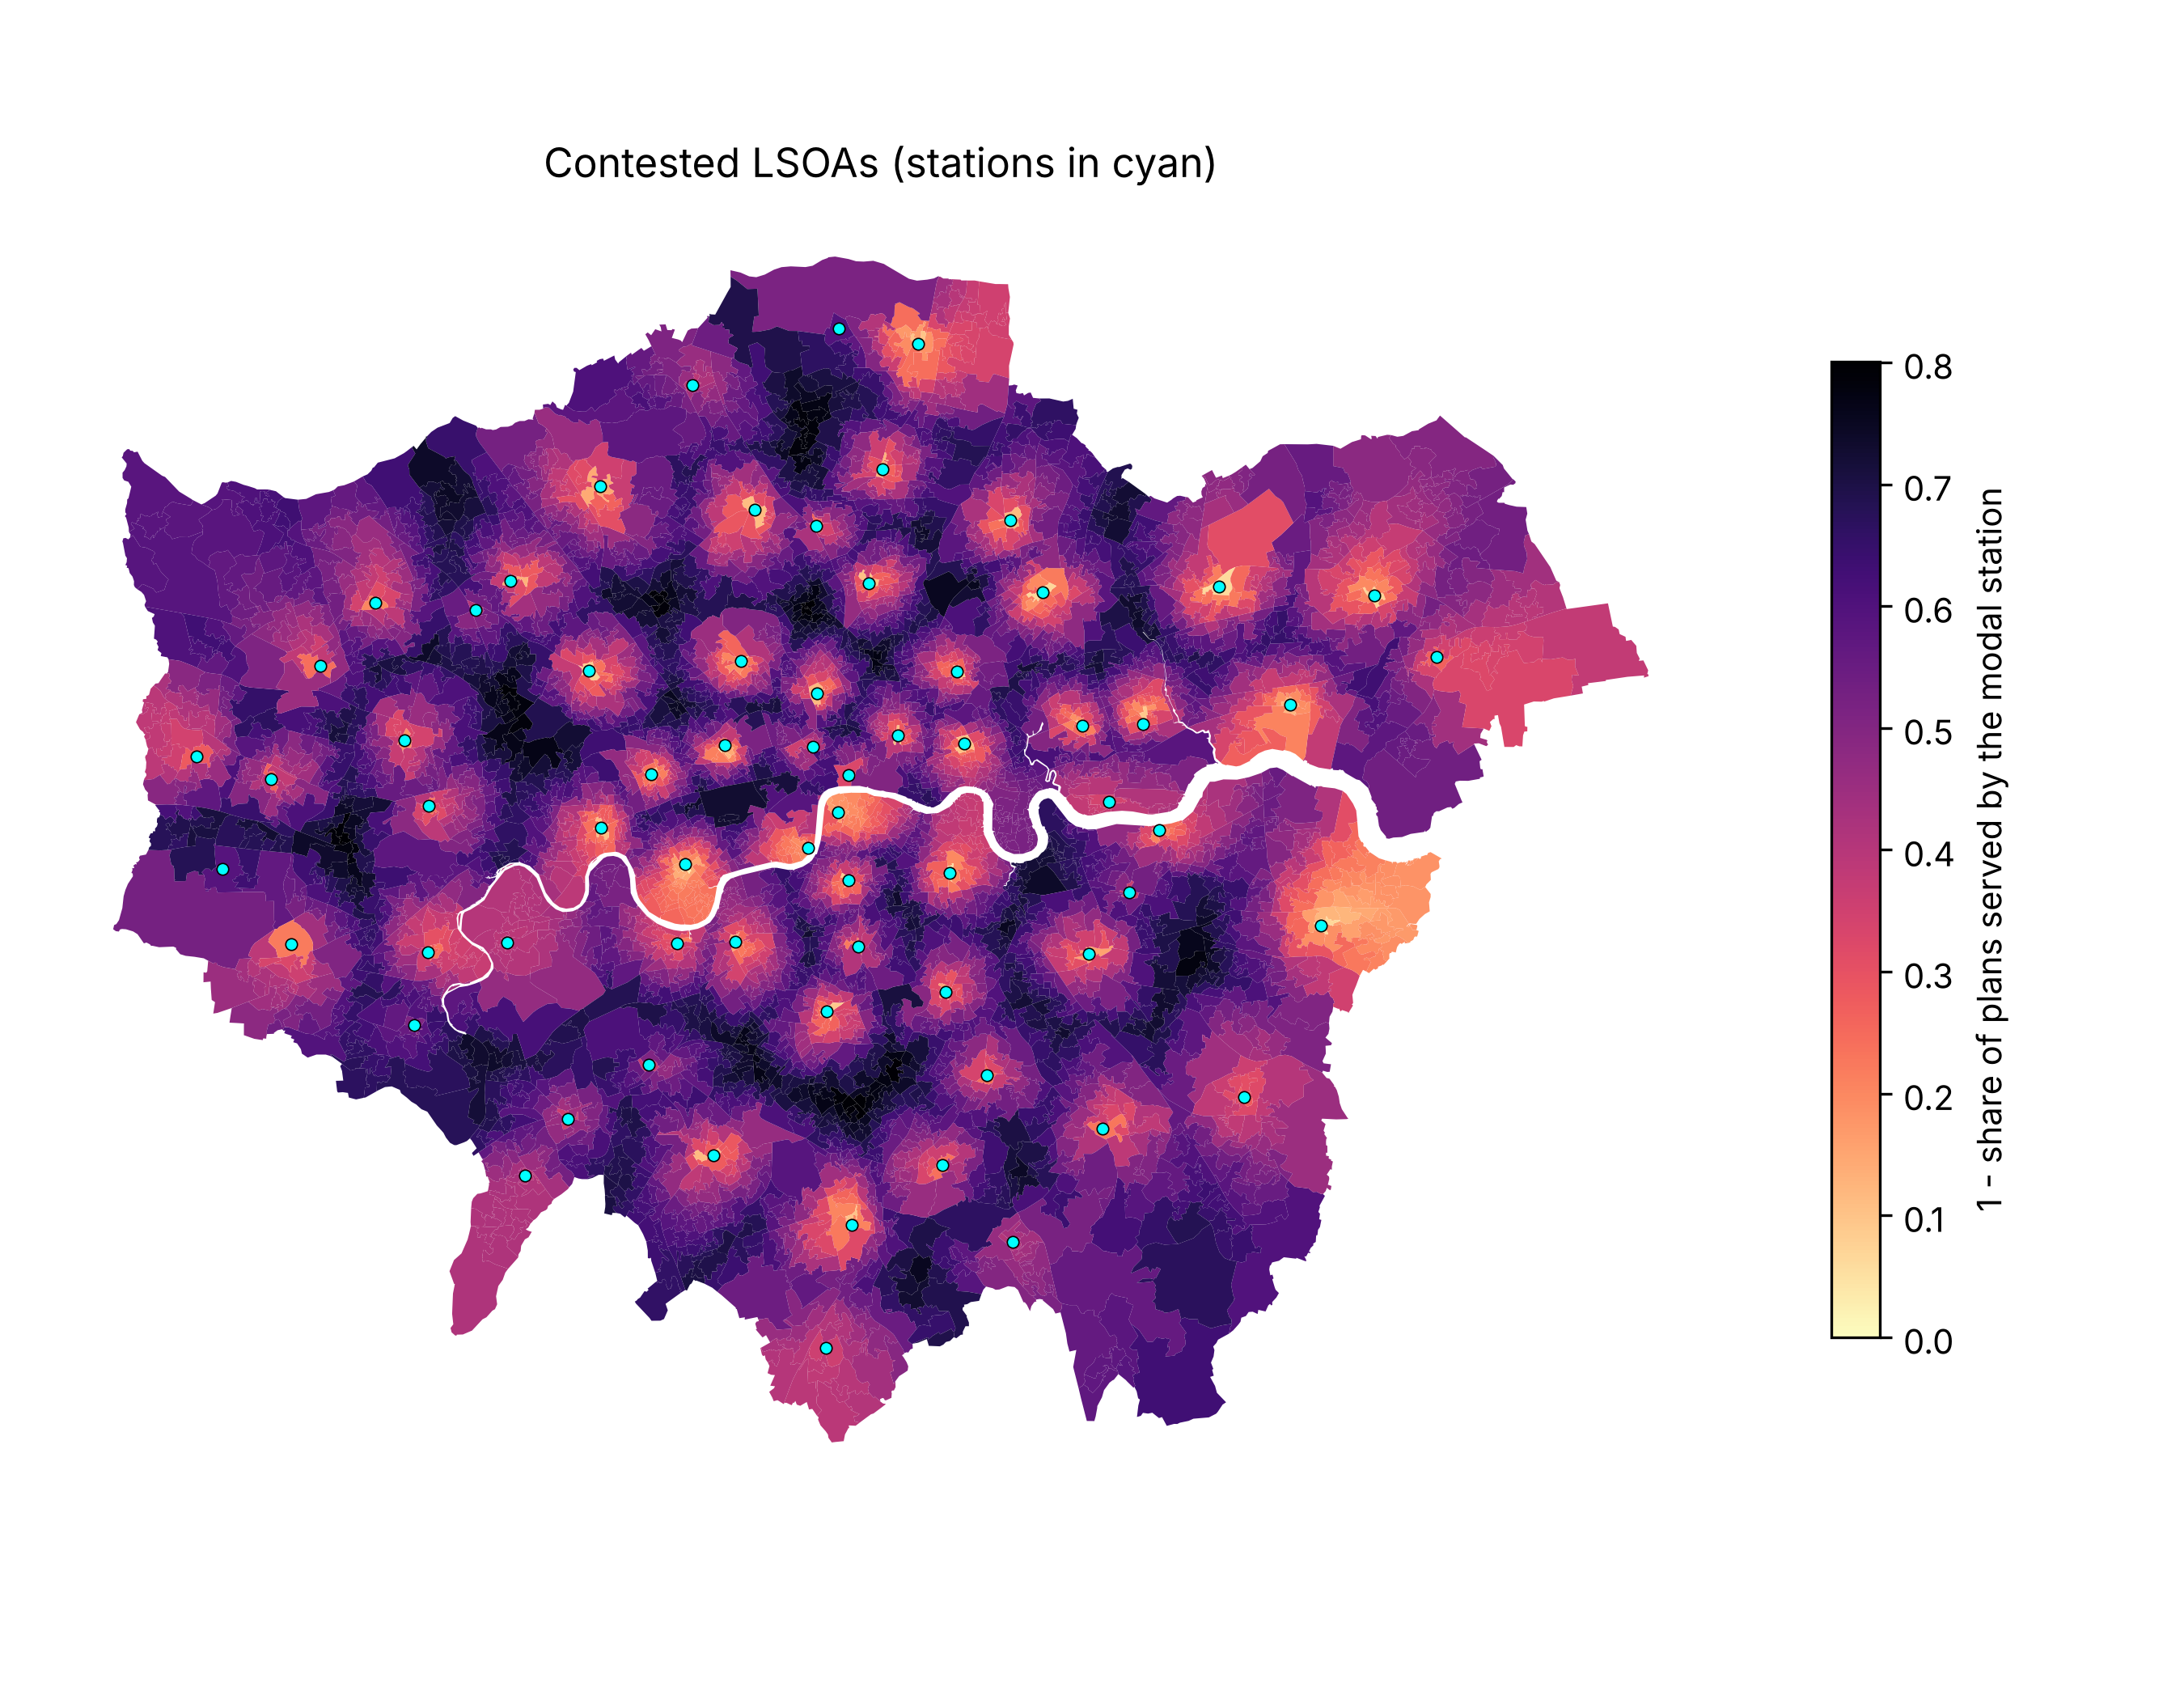
\includegraphics[width=\linewidth]{figures/las/fig_contested.png}
  \caption{Contestedness of each LSOA: one minus the share of plans in which it is served by its most frequent station.}
  \label{fig:las-contested}
\end{subfigure}
\caption{Boundaries and contested areas in the pooled ensemble. In (\subref{fig:las-boundary-panels}) darker and thicker edges are cut more often, and the colour scale runs to the largest observed frequency. Stations are marked in (\subref{fig:las-contested}).}
\label{fig:las-boundary}
\end{figure}

\paragraph{Stations.}
Because the candidates are the real stations, the ensemble also describes each station (Figure~\ref{fig:las-stations}). A plan opens $52.5$ stations on average, between $43$ and $61$, and between $49$ and $56$ in the central $90\%$ of plans. Seventeen stations are open in more than $90\%$ of plans, led by Fulham ($97\%$) and St John's Wood ($96\%$). No station is open in fewer than $40\%$ of plans, and the median station is open in $83\%$. The least used sites are those whose surroundings cannot fill a unit or that sit next to a stronger neighbour: Chase Farm ($40\%$), Heathrow Airport ($41\%$) and Twickenham ($49\%$). An open frequency counts how often the law opens a station. It says nothing about the cost of closing one, which the ensemble does not measure. Capacity follows density: over all open stations $42\%$ carry one unit, $31\%$ two and $27\%$ three; inner stations such as St John's Wood, Ilford and Camden carry three units in about $40\%$ of the plans in which they are open, and outer stations such as Tolworth, Richmond and Chase Farm carry one unit in about $70\%$ of theirs.

\begin{figure}[!htbp]
\centering
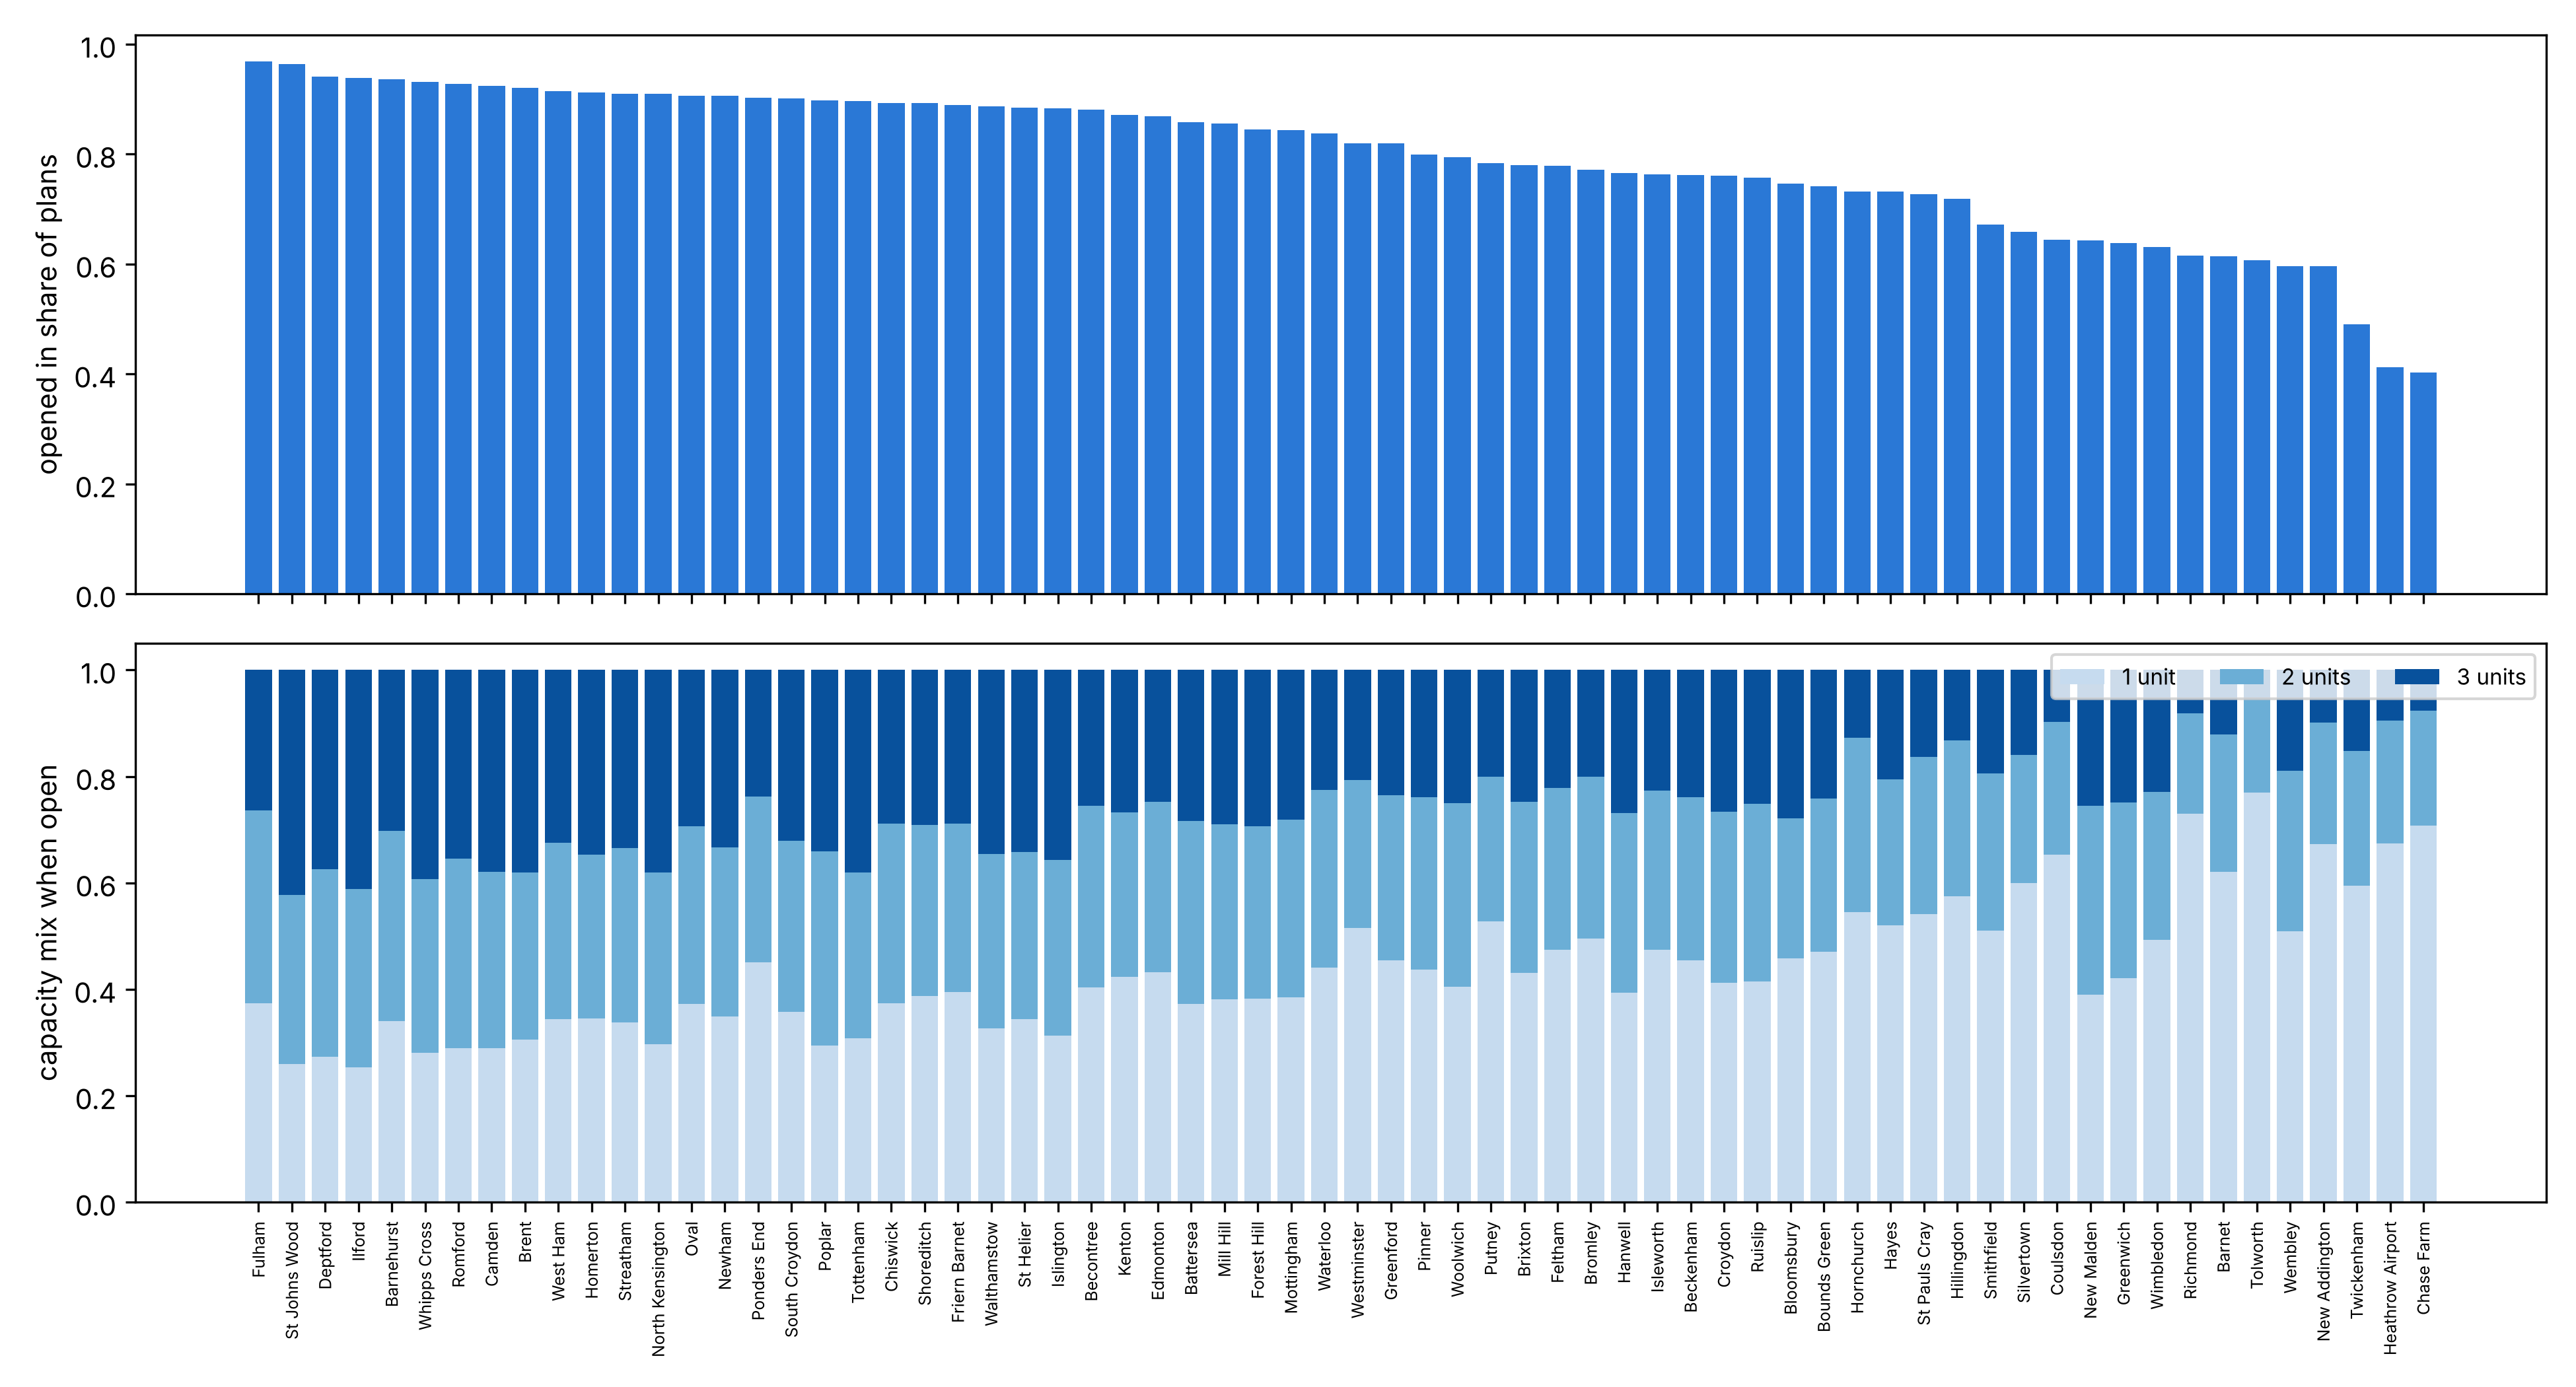
\includegraphics[width=\linewidth]{figures/las/fig_stations.png}
\caption{Top: share of plans in which each station is open, sorted. Bottom: capacity mix of each station in the plans in which it is open.}
\label{fig:las-stations}
\end{figure}

\paragraph{Groups.}
The sampled Groups recover part of the operational structure (Figure~\ref{fig:las-groups}). A plan has $22.3$ Groups on average, between $20$ and $24$ in the central $90\%$ of plans, against the $21$ real Groups. Two stations of the same real Group share a superdistrict in $27\%$ of the plans in which both are open, two stations of different Groups in $2\%$; part of this contrast is distance. The adjusted Rand index between a sampled grouping of the open stations and the real Groups is $0.28$ on average ($0.17$ to $0.39$ in the central $90\%$ of plans), against $0.19$ between two sampled plans from different chains. The real Groups are thus one contiguous, capacity-feasible grouping among many that the geography admits, a typical member of the family and not its mode. The pairs the ensemble keeps together most often inside a real Group are Hornchurch and Romford ($67\%$) and Barnehurst and Woolwich ($55\%$). Equally strong are pairs that the real Groups separate, such as Barnehurst and St Pauls Cray ($49\%$) and Richmond and Putney ($48\%$); fourteen cross-Group pairs exceed $30\%$, against $29$ within-Group pairs. These are the associations a planner would examine first, since they mark Group boundaries that balanced plans tend not to draw.

\begin{figure}[!htbp]
\centering
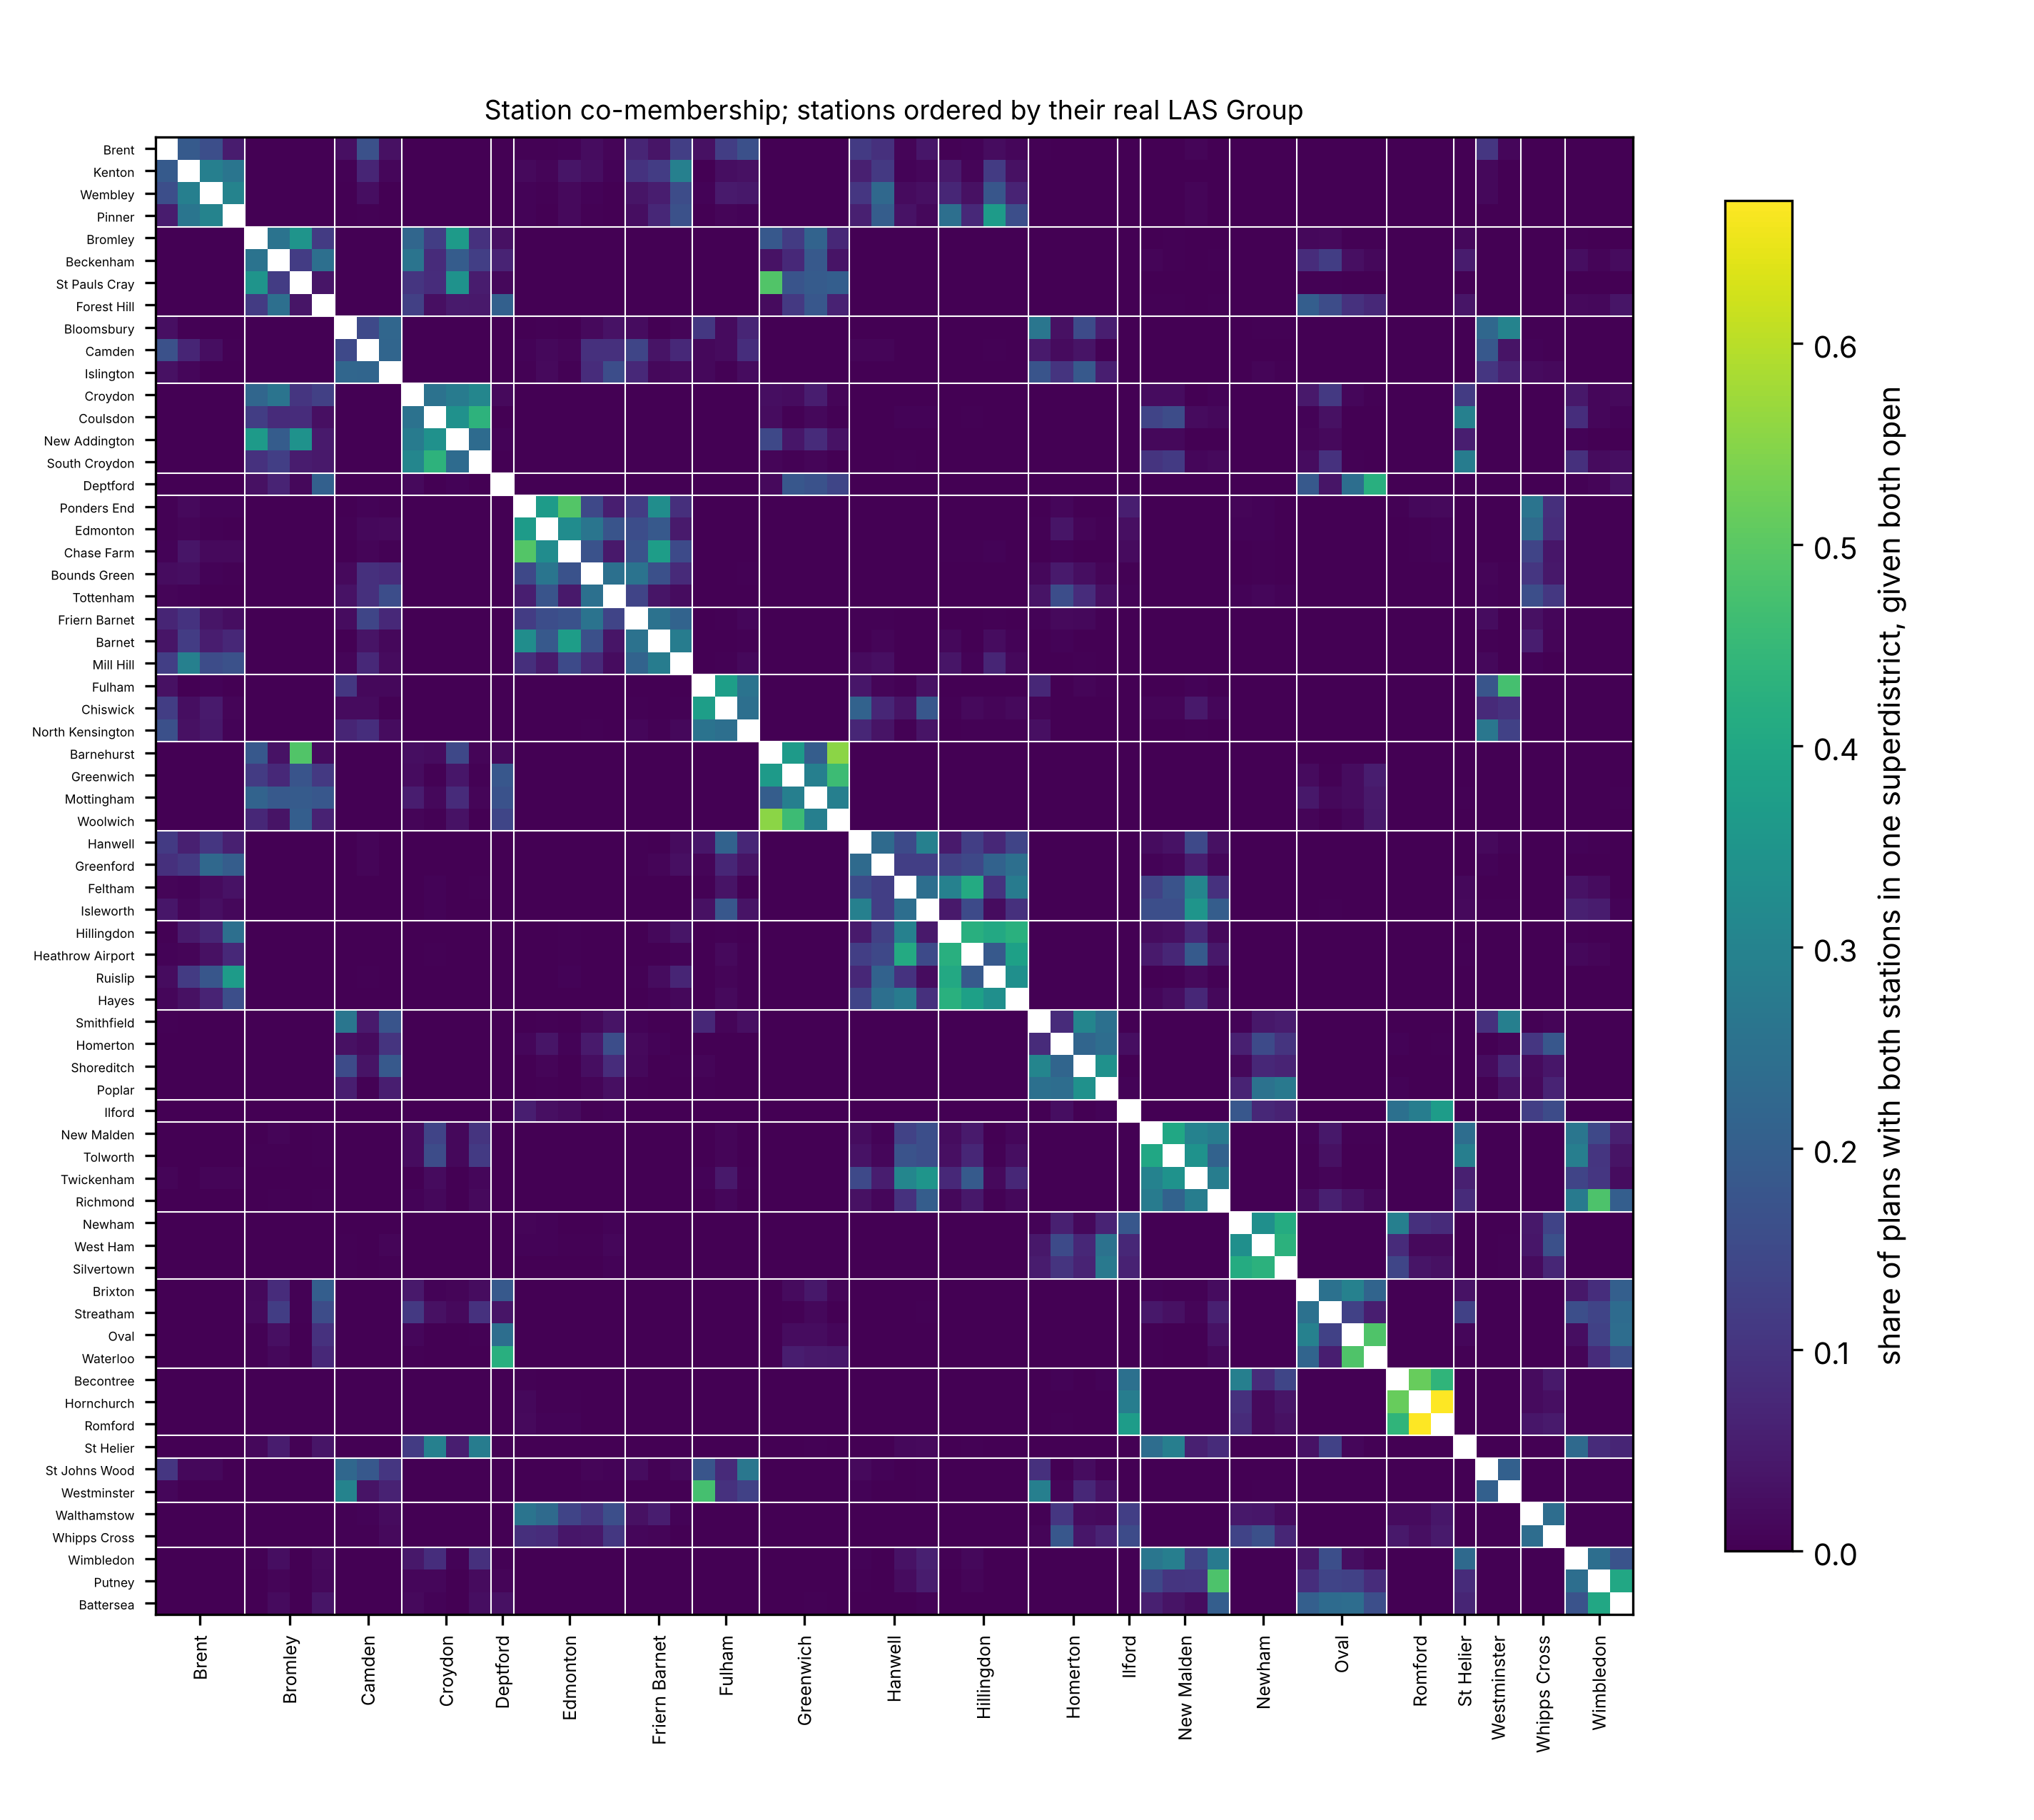
\includegraphics[width=0.7\linewidth]{figures/las/fig_groups.png}
\caption{Share of plans in which two stations belong to the same superdistrict, among the plans in which both are open; stations ordered by their real Group, with white lines separating the $21$ Groups and the colour scale running to the largest off-diagonal value.}
\label{fig:las-groups}
\end{figure}

% -------------------------------------------------------------------------
\FloatBarrier
\subsection{The Operational Layout Against the Ensemble}\label{sec:las-price}
% -------------------------------------------------------------------------

\emph{Finding.} The operational layout has a lower access cost than every one of the $6{,}400$ sampled plans and than every annealed plan. The reason is its station loads, $20$ of which lie outside every balance window. The distance from the layout to the best balanced plan found, $0.5$ minutes of mean drive time, is an upper bound on the access cost of workload balance at this calibration.

\begin{table}[!htbp]
\centering
\small
\begin{tabular}{lrrrrr}
\toprule
 & open & station-leg energy & mean drive & $90$th pct. & within \\
plan & stations & [million min] & time [min] & [min] & $8$ min [\%] \\
\midrule
operational layout $s_{\mathrm{LAS}}$ & $66$ & $3.08$ & $2.92$ & $4.78$ & $99.5$ \\
\midrule
ensemble, mean & $52.5$ & $4.22$ & $3.99$ & $6.98$ & $94.5$ \\
\quad central $90\%$ & $49$--$56$ & $4.00$--$4.47$ & $3.78$--$4.23$ & $6.46$--$7.56$ & $91.8$--$96.7$ \\
best sampled plan & $56$ & $3.75$ & $3.55$ & $6.08$ & $97.5$ \\
best annealed plan & $55$ & $3.63$ & $3.44$ & $5.90$ & $98.8$ \\
\midrule
bound: annealed $-$ layout & & $0.55$ & $0.52$ & $1.12$ & $-0.8$ \\
\bottomrule
\end{tabular}

\caption{The operational layout against balanced plans, on the station leg. ``Best sampled plan'' is the stored plan with the lowest station-leg energy; ``best annealed plan'' is the best of eight annealing runs of $50{,}000$ steps. The last row is the upper bound on the access cost of workload balance.}
\label{tab:las-layout}
\end{table}

\begin{figure}[!htbp]
\centering
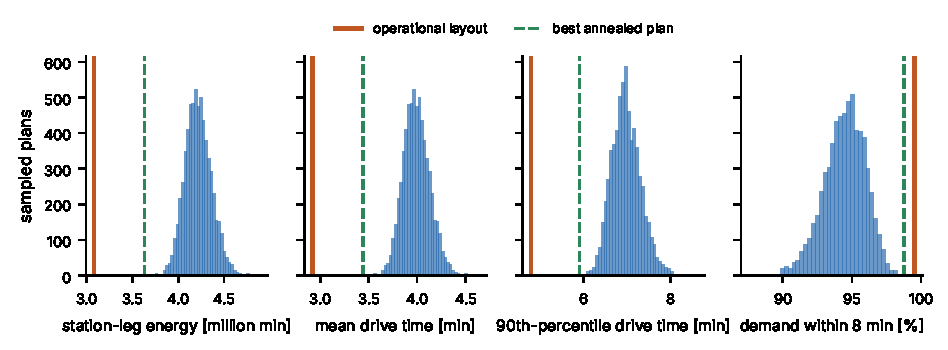
\includegraphics[width=\linewidth]{figures/sec7/fig_layout_vs_ensemble.pdf}
\caption{Station-leg metrics of the $6{,}400$ sampled plans, with the operational layout and the best annealed plan.}
\label{fig:las-slas}
\end{figure}

\paragraph{Position.}
Table~\ref{tab:las-layout} and Figure~\ref{fig:las-slas} place the operational layout in the ensemble. Its station-leg energy is $3.08$ million demand-weighted minutes, below the lowest of the stored plans ($3.75$ million) and $27\%$ below the ensemble mean. Its mean drive time is $2.9$ minutes against $4.0$ in the ensemble, its $90$th percentile $4.8$ minutes against $7.0$, and $99.5\%$ of its demand lies within eight minutes' drive of its catchment station against $94.5\%$.

\paragraph{Source: the station loads.}
The operational layout opens all $66$ stations, where the sampled plans open $43$ to $61$, and its loads range from $0.19$ to $4.68$ units, a factor of $25$ (Figure~\ref{fig:las-loads}). Measured against the widest windows the chain can produce, $20$ of the $66$ stations fall outside. Ten serve less than $0.72$ units, among them Waterloo at $0.19$ and Smithfield and Heathrow Airport at about $0.5$; Deptford, at $4.68$, exceeds the three-unit range; and nine fall between the one-unit and two-unit ranges, loads that blocks of three ambulances cannot express. Against the nominal $\pm15\%$ windows of the model the count is $36$. None of these statements depends on the sampled law.

\begin{figure}[!htbp]
\centering
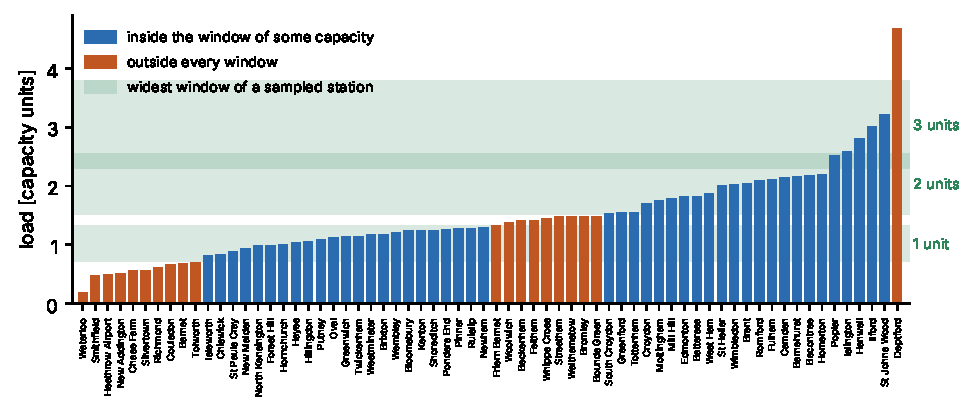
\includegraphics[width=\linewidth]{figures/sec7/fig_station_loads.pdf}
\caption{Station loads of the operational layout in capacity units, sorted. The bands are the widest load windows that a sampled station of one, two or three units can have (Proposition~\ref{prop:effective}).}
\label{fig:las-loads}
\end{figure}

\paragraph{An upper bound on the price of balance.}
Every sampled plan satisfies the windows, so the minimum access cost over the balanced plans lies at or below that of the best plan we can exhibit, and the distance from that plan to the operational layout bounds the access cost of workload balance from above. The best stored plan gives a bound of $0.67$ million demand-weighted minutes, $22\%$ of the layout's station leg. The sample minimum is a loose bound, since the chain does not seek low energy (Section~\ref{sec:exp-milp}). To tighten it we run the annealing mode of Section~\ref{sec:exp-milp} on this instance, eight seeds of $50{,}000$ steps with the calibration unchanged, $43$ to $53$ minutes per seed. The best annealed plan opens $55$ stations and tightens the bound to $0.55$ million minutes, $18\%$ of the layout's station leg: $0.5$ minutes of mean drive time, $1.1$ minutes at the $90$th percentile and $0.8$ points of eight-minute share (Table~\ref{tab:las-layout}). The operational layout remains below every balanced plan found, and the bound remains an upper bound, which a better optimizer would lower further.

\paragraph{Reading the bound.}
Part of this price is a limit of the demand proxy and not of the layout: the smallest catchments sit on daytime hot spots, the West End, the City and the airport, which residential apportionment does not see. Whether the rest is worth paying is an operational question that the ensemble informs but does not settle.

% -------------------------------------------------------------------------
\FloatBarrier
\subsection{Sensitivity to the Demand Proxy and the Tolerance}\label{sec:las-sensitivity}
% -------------------------------------------------------------------------

\emph{Finding.} Under a second demand proxy and under a wider tolerance the station-level frequencies move by a few points, and the structure of the ensemble and the position of the operational layout below it do not change.

We repeat the study twice (Table~\ref{tab:las-sens}). In the first replication each borough's incidents are spread uniformly over its LSOAs instead of in proportion to population, the crudest alternative, with the same calibration and protocol. In the second the tolerance is $\varepsilon^1 = \varepsilon^2 = 0.25$, the widest that keeps the debt windows of the recursion disjoint with margin (Claim~\ref{claim:app-unique} allows up to $2/5$), with four chains of $40{,}000$ steps.

\begin{table}[!htbp]
\centering
\small
\resizebox{\linewidth}{!}{\begin{tabular}{lrrr}
\toprule
 & baseline & uniform demand proxy & $\varepsilon^1=\varepsilon^2=0.25$ \\
\midrule
chains $\times$ steps & $4\times80{,}000$ & $4\times80{,}000$ & $4\times40{,}000$ \\
acceptance & 67.7--68.0\% & 67.6--68.2\% & 70.0--70.6\% \\
largest KS between chains (access cost, $|\Pc^1|$, cut edges) & $0.078$, $0.037$, $0.070$ & $0.033$, $0.062$, $0.037$ & $0.079$, $0.053$, $0.098$ \\
\midrule
open stations, mean (range) & $52.5$ ($43$--$61$) & $52.5$ ($44$--$62$) & $53.3$ ($47$--$62$) \\
stations open in more than $90\%$ of plans & $17$ & $16$ & $21$ \\
Groups per plan, mean & $22.3$ & $22.3$ & $22.5$ \\
adjusted Rand index against the real Groups & $0.28$ & $0.28$ & $0.28$ \\
\midrule
station-leg energy, ensemble mean [million min] & $4.22$ & $4.23$ & $4.22$ \\
\quad lowest stored plan & $3.75$ & $3.77$ & $3.79$ \\
\quad operational layout & $3.08$ & $3.10$ & $3.08$ \\
mean drive time, ensemble / layout [min] & $4.0$ / $2.9$ & $4.0$ / $2.9$ & $4.0$ / $2.9$ \\
demand within $8$ min, ensemble / layout & $94.5\%$ / $99.5\%$ & $94.4\%$ / $99.5\%$ & $94.4\%$ / $99.5\%$ \\
\midrule
layout stations outside every window (of $66$) & $20$ & $20$ & $6$ \\
\quad outside the nominal $\pm\varepsilon$ windows & $36$ & $39$ & $26$ \\
layout below every sampled plan & yes & yes & yes \\
\bottomrule
\end{tabular}
}
\caption{The London study under the baseline, under a uniform within-borough demand proxy, and under a tolerance of $0.25$. ``Outside every window'' counts the stations of the operational layout whose load lies outside the widest window of every capacity at the tolerance of the column.}
\label{tab:las-sens}
\end{table}

\paragraph{Demand proxy.}
The open frequency of a station moves by at most $0.09$ between the two proxies (mean $0.01$), with a single station moving by more than $0.05$: Heathrow Airport, from $41\%$ to $33\%$ once the airport's demand is spread over its borough. The set of stations open in more than $90\%$ of plans exchanges five stations that lie within $0.03$ of the threshold. The frequencies move, as they must when the demand surface moves, but the number of open stations, the recovery of the real Groups and the position of the layout do not.

\paragraph{Tolerance.}
At $\varepsilon = 0.25$ the plans open slightly more stations and the mean station-leg energy is within $0.1\%$ of its value at $0.15$. The run is half as long and its diagnostics are correspondingly weaker (Appendix~\ref{app:london-extra}). The wider windows admit $14$ of the layout's $20$ out-of-window stations, but six remain outside, five below $0.56$ units and Deptford above $4.38$. The gap to the layout thus comes from the capacity model itself, in which every open station serves between $0.56$ and $4.4$ units in blocks of three ambulances, whereas the operational layout runs stations from $0.19$ to $4.68$ units. A calibration that lets a plan keep both its smallest and its largest stations needs a wider capacity range, which by Corollary~\ref{cor:app-invariant} means a larger block or the rejection-based treatment of $c \ge 4$.

\paragraph{Scope of the case study.}
All figures are drive times of a static assignment of every LSOA to a catchment station. Real dispatch sends the nearest available vehicle, and LAS balances workload dynamically, so the figures describe catchment geometry and not response performance; the published response-time clock, which includes call handling and mobilisation, offers no validation of them. A uniform speed factor rescales every drive time and leaves the ordering of plans and the ratio of the layout's energy to the ensemble's unchanged, but not the eight-minute share. The comparison is between a contiguous hierarchical layout and a sample of plans that satisfy constraints the layout does not.
